% !TEX root = ../report.tex

\chapter{Electrical}\label{electrical}

\section{Power Distribution and Motor Drive}\label{elec/poweranddrive}
The Pololu Power Distribution and Motor Drive board~\cite{pololupower}
was selected for power distribution across
the robot. This board is the main accompanying part for the Romi
chassis chosen, and in addition to power distribution also provides
two Texas Instruments DRV8838~\cite{texasdrivers} motor drivers to control the motors. The board integrates with the chassis easily
and regulates the voltage provided by the 6 AA batteries, using an
MP4223H switching buck converter~\cite{mpbuck}, to \SI{5}{\volt} or
\SI{3.3}{\volt} at a maximum of \SI{2.5}{\ampere}. This can be used
to power the microcontroller and peripherals used by the robot, with the motors being supplied with the reverse protected voltage before
regulation.

The board was also configurable if required, allowing the supply to be
divided into \SI{4.8/6}{\volt} and \SI{2.4/3}{\volt} supplies dependent on the voltage of the batteries used.
There are also a number of further jumper connections on the board which can
be cut for further voltage customisation.

The DRV8838 Motor Driver takes two inputs for each motor for direction and Pulse Width
Modulation (PWM), which allows the motor speed to be controlled. The
driver also has a sleep input which can be used to coast the motors if
this would be beneficial. Each of the motors' respective sleep inputs
and are connected by default and therefore should not be driven at the same time, as this could result in short cases within the motor driver, however
the jumper connection between these can be cut to allow the sleep inputs to
be driven separately.

The power board also provides a power button and switch to control the
power supply. A separate board with only power distribution was
available, however, for the additional small cost, integration of
motor drivers was deemed to be a cost effective addition given our space and time limitations.

The boards were soldered to the battery contacts and headers soldered
onto the boards as the robots were assembled. Once soldered, the power distribution board and 
motor driver board were continuity tested.

\section{Range Sensors}\label{elec/range}
For the robot to localise itself, it needs to be able to measure the
distance between itself and the surrounding environment. By recording
the measurements relative to the robots current position, a point map
can be built up over time and a general map of the environment can be
constructed.

\subsection{Design}\label{elec/range/design}
Infra-red, ultrasound and LIDAR distance sensors were all considered. These
are all active sensors, meaning that they measure the effect of an
output from the sensor, in these cases, IR light, ultrasonic waves
and visible light respectively.

Of these three, LIDAR is generally considered to be the most effective
as it is the most accurate and has a \ang{360} field of view. However,
it is both too expensive and too heavy for our application, especially
considering the scalability requirement of the project. 

Infra-red transceivers are far more affordable but have a limited cone of 
vision per sensor as light deviates very little through air and the 
maximum range of these sensors is approximately \SI{0.5}{\m}~
\cite{InfraredDatasheet}. Ultrasonic transceivers have a wider cone of 
detection and also a large range~\cite{HCSR04datasheet}. In addition to 
this, they are also cheaper than both infra-red and LIDAR systems. 

Ultrasonic transceivers were therefore decided upon for use in this
project. These work by transmitting sound at a particular frequency
and measuring the time until the reflected wave returns to the sensor. 
Ultrasonic sensors have the chance to interfere with each other, 
however, infra-red could also interfere with each other and are also 
more likely to be affected by external interference. A possible solution 
was to make a cheap LIDAR unit using a single infra-red sensor and a 
servo motor mounted on top of the robot. This was, however, dismissed as 
the two PWM pins of the Raspberry Pi would be assigned to each of the 
motors respectively. This solution would also require a budget and 
software implementation commitment prior to testing which was not deemed 
worth the potential added risk to the project.   

Hence ultrasonic sensors were chosen and the ultrasonic sensor used was 
the HC-SR04~\cite{HCSR04datasheet}, as previously mentioned in Section~
\ref{mech/sensors}. This sensor has a range of up to \SI{4}{\m} and 
ranging accuracy of up to \SI{3}{\mm}. A small dead-band exists in its 
range at $<$~\SI{30}{\mm}, however this is mitigated by the placement of 
the sensor $\approx{\SI{30}{\mm}}$ from the edge of the robot chassis. 


The sensor is also widely used and available within the 
department, mitigating any risks surrounding delivery lead times. 

\begin{figure}[!ht]
	\centering
	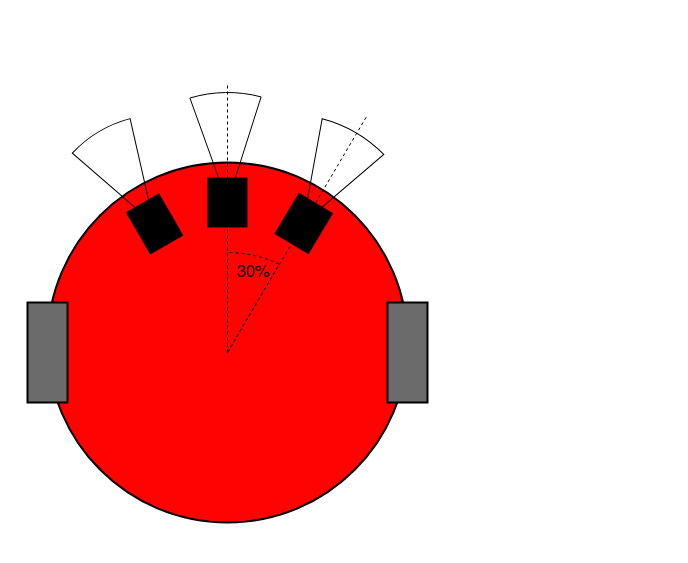
\includegraphics[width=0.5\textwidth]{diagrams/UltraSoundSensorDiagram.png}
	\caption{Ultrasound Sensor Layout}\label{UltraSoundSensorDiagram}

\end{figure}

\subsection{Implementation}\label{elec/range/impl}
The hardware required for the ultrasonic sensors is relatively straightforward. 
They are each connected to a \SI{5}{\volt} supply and ground, and the other two pins are 
connected to standard GPIO pins on the RPi. The echo pin has to be connected through 
a voltage divider as the RPi is only rated at \SI{3.3}{\volt} compared to the sensor's \SI{5}{\volt}. The 
trig pin can be connected directly to the RPi, however, as \SI{3.3}{\volt} was found to be above 
the threshold voltage.

The distances are measured by an \textit{USScan} class. This has a \textit{get
\_scan()} function which iterates through each ultrasonic sensor and takes a reading, 
as shown below in Code Listing \ref{lst:get_scan}.

\begin{lstlisting}[caption={get\_scanFunction in USScan},label={lst:get_scan} , language=python]
def get_scan():
    """Get scan of ranges from all ultrasonic sensors.
    :return: (USScan) Scan of ranges
    :except: (UltrasonicTimeout) If module timed out waiting for GPIO input change
    """
    start = time.time()
    rl = get_range(LEFT)
    time_remaining = start + scan_increment - time.time()
    if time_remaining > 0:
        time.sleep(time_remaining)
    rc = get_range(CENTRE)
    time_remaining = start + 2 * scan_increment - time.time()
    if time_remaining > 0:
        time.sleep(time_remaining)
    rr = get_range(RIGHT)
    return USScan([rl, rc, rr])
\end{lstlisting}

This method allows the various readings to be taken without interfering with each other, as the second ultrasonic pulse isn't omitted until the first is received.

As \ref{lst:get_scan} shows,\textit{get\_range()} is used by
\textit{get\_scan()} to find the distance measured by each sensor.
This simply triggers the sensor and times how long until the echo
pin turns high. The range is then calculated by the equation
$ 2d = tv_s$ where $v_s$ is the speed of sound. It is then converted
to mm.

\subsection{Testing}\label{elec/range/test}
The sensors were initially tested using a signal generator and an
oscilloscope. An object was then placed in front of the sensors
and moved away. The expected output of this test was a linear increase
in the width of the pulse width on the echo pin as the distance
increased. This experiment allowed us to quickly identify 2
malfunctioning sensors. The pulse width could then be used to to
calculate the measured distance and this compared to the distance
found with a measuring tape. This found approximately correct answers,
however the precision with which we could measure the pulse width was
not great enough for effective testing.

The wave forms produced are shown in Figure~\ref{UltrasoundWaveform}.
This shows the shorted echo pulse following the fall of the wider
square wave on the trig pin, produced by the signal generator.

\begin{figure}[!ht]
	\centering
	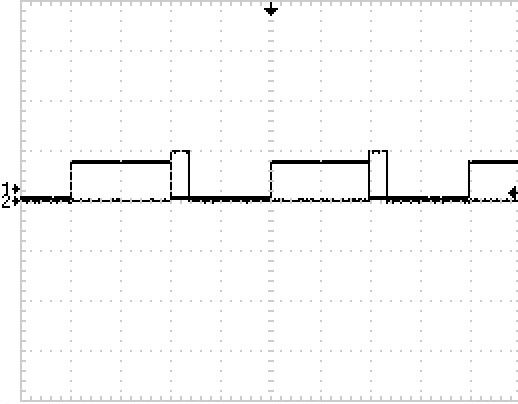
\includegraphics[width=0.5\textwidth]{graphs/UltrasonicResponseGraph.jpg}
	\caption{Ultrasound Response Waveform}\label{UltrasoundWaveform}

\end{figure}

A circuit was then created to read the values using an Arduino
microcontroller to allow the distance readings to be found quickly
and the accuracy of the sensors measured. The readings from this were
found to be approximately accurate (to at least within a half a cm,
as measured with a tape measure), although rigorous testing was not
performed as the accuracy would be dependant on the temperature due
to changes in air pressure, and we had no way of accurately controlling
this.

The testing was then repeated using the RPi set-up as to test the
software, with similar results obtained.

\section{Encoders}\label{elec/encoder}
Wheel encoders are required to measure the speed of each wheel
independently. This gives the system far more control over its path
as well as allowing it to perform dead reckoning through wheel odometry.

\subsection{Design}\label{elec/encoder/design}
The motors selected had both incremental and absolute custom designed
encoder, but as only the wheel speed is needed and not the position,
the incremental rotary encoders were used. These were hall effect
encoders, which measure the changing magnetic field of magnets which
are attached to the motor shaft. It has two 6 pole magnets magnets
which create 12 counts per revolution of the motor shaft, which, after
scaling for the gear ratio of 120:1, results in 1440 counts per
revolution of the robot wheel.

The encoders are quadrature encoders, which represent the speed and
direction of the wheels with two square waves where the frequency
represents the speed and which of the two waves is leading shows the
direction.

\subsection{Implementation}\label{elec/encoder/impl}

The encoder data was read into the RPi by an encoder class written in
Python. This worked by connecting call back methods to both the A and B
channel pins. How this is initialised is shown in Code Listing
\ref{lst:enc_event_detect}

\todo{format listings}

\begin{lstlisting}[caption={encoder callback set-up},label={lst:enc_event_detect} , language=python]
GPIO.add_event_detect(self.pin$_$a, GPIO.BOTH, callback=self._callback_a)
\end{lstlisting}

This then either increments or decrements a count depending on the
direction, as shown in Code Listing \ref{lst:enc_callback}. Note that
\textit{\_callback\_b()} is identical but with \textit{self.\_inc()} and
\textit{self.\_dec()} switched.

\begin{lstlisting}[caption={Encoder Callback Function},label={lst:enc_callback} , language=python]
def _callback_a(self, _):
        a, b = GPIO.input(self.pin_a), GPIO.input(self.pin_b)
        if a == b:
            self._inc()
        else:
            self._dec()
\end{lstlisting}


\subsection{Testing}\label{elec/encoder/test}
The encoders were first tested to ensure that they functioned correctly
using a test circuit and connecting the encoder outputs to an
oscilloscope. All the encoders were shown to function correctly
outputting square waves in both channels and with channel A leading B
when the motor was moving forwards and B leading A when going forwards.
\todo{check order}

An example of the encoder output found is shown in Figure
\ref{EncoderGraph} below. This shows the two square waves produced by the
two encoder outputs a quarter wavelength out of phase.

\begin{figure}[!ht]
	\centering
	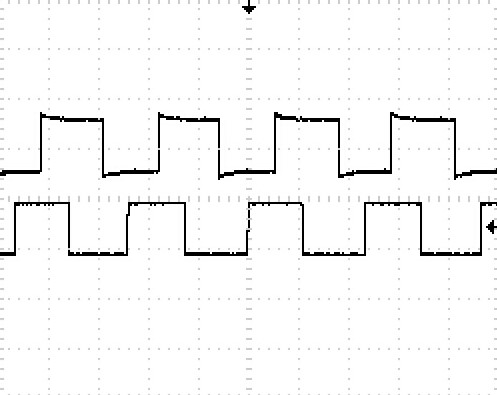
\includegraphics[width=0.5\textwidth]{graphs/EncoderGraph.jpg}
	\caption{Encoder Output Test Waveforms}\label{EncoderGraph}

\end{figure}

This experiment allowed us to quickly confirm the correct functionality
of all 6 encoders, however did not allow us to test the accuracy. After
this, the motors were run at a low speed for several rotations while the
system counted pulses. This was not an accurate test of the encoders, as
the wheel could not be stopped at an exact integer multiple of rotations,
however did verify that the system was approximately outputting 1440
counts per rotation.

\section{IMU}\label{elec/imu}
The IMU consists of a three axis accelerometer and a three axis gyroscope
which can be used to measure both the linear acceleration and rotational
velocity of the robot. This can be integrated and double integrated to
track the robots position over time again performing dead reckoning. The
system can then perform sensor fusion on this data and the encoder
readings to get far more accurate results than possible with either system
independently.

\subsection{Design}\label{elec/imu/design}
The IMU selected was the MPU-6050. It was the most accurate sensor of a
similar budget with regards to noise, cross axis sensitivity and non
linearity. Offset tolerance was also considered but this was less of a
consideration as this can be compensated for as long as the offset is not
so extreame as to limit the range. It was configured to operate in its
smallest range of values ($\pm\ang{250}s^{-1}$ and $\pm2g$~\cite{MPU6050Datasheet}).

The IMU was to be placed as close to the centre of the axis of the robot
as possible, as when it is far from the centre of rotation the centripetal
forces acting on it can interfere and be measured as linear motion away
from the centre.

\subsection{Implementation}\label{elec/imu/impl}
The IMU selected uses the I$^2$C protocol for data transmission, which
integrates well with the RPi as it has dedicated I$^2$C GPIO pins and
existing libraries to facilitate communication.

It should be noted that, while this was the only I$^2$C device currently
used, other devices with conflicting addresses can be handled as The IMU
allows the address to be changed through a data pin from 0x68 to 0x69.
This would most likely be used if the framework developed was being used
on another, more complicated system requiring several IMUs. This pin was
not connected to the RPi in this design as it was not yet required.
\todo{code description}

An \verb|i2c_object| class that used the smbus package was created to
simplify the communication over the I\textsuperscript{2}C buses. These
were initialised with an I\textsuperscript{2}C bus and an address, and
contained various methods for reading and writing to the I
\textsuperscript{2}C device.

\todo{what code is interesting}

An \verb|IMU| class was then created to read the data from the IMU which
and an \verb|i2c_object| instance. Code Listing \ref{lst:imu_init} shows
the constructor for the IMU class. Note that the \verb|write_byte()| call
is essential to enable the IMU transmissions.

\begin{lstlisting}[caption={IMU Initialisation Function},label={lst:imu_init} , language=python]
def __init__(self, address, rate, channel=1):
    self.address = address
    self.IMU_i2c = i2c.i2c_object(self.address, channel=channel)
    self.rate = rate
    self.IMU_i2c.write_byte(0x6B, 0x00) # turns imu on
    self.speed_vect = (0.0, 0.0, 0.0)
\end{lstlisting}

As the IMU returns arbitrary values between -32768 and 32767~\cite{MPU6050Datasheet}, a constant was required to convert the results to
meaningful values. The calculations for these is shown in Code
Listing~\ref{lst:imu_units}.

\begin{lstlisting}[caption={Calculation for IMU Value to SI unit Conversion Constants},label={lst:imu_units} , language=python]
GYRO_RANGE = 250  # deg/sec
GYRO_DIVISIONS = 32768  # 2 ^15
GYRO_UNITS = (GYRO_RANGE * math.pi * 2.0) / (GYRO_DIVISIONS * 360)  # rad/sec

ACC_RANGE = 2 * 9.81  # m/s^2
ACC_DIVISIONS = 32768  # 2 ^15
ACC_UNITS = ACC_RANGE / ACC_DIVISIONS  # m/s^2
\end{lstlisting}

The acceleration values can then be multiplied by the \verb|ACC_UNITS|
constant and the result is the acceleration in $ms^{-2}$, and \verb|GYRO_UNITS|
can be used similarly to find the rotation in $rads^{-1}$, as is
shown in Code Listing \ref{lst:read_funcs}.


\begin{lstlisting}[caption={Reading and Converting Raw IMU Values},label={lst:read_funcs} , language=python]
    def _read_gyro(self):
        x_rot_v = self.IMU_i2c.read_signed_word(0x43) * GYRO_UNITS
		...
        return (x_rot_v, y_rot_v, z_rot_v)

    def _read_accel(self):
        x_a = self.IMU_i2c.read_signed_word(0x3b) * ACC_UNITS
		...
        return (x_a, y_a, z_a)
\end{lstlisting}

The final step in reading the IMU results is to integrate the acceleration
data as to get the linear velocities. This makes use of the \textit{speed
\_vect} variable declared in the IMU constructor shown in Code Listing
\ref{lst:imu_init}. \textit{speed\_vect} is incremented by the
acceleration multiplied by the IMU rate, as shown in
\ref{lst:imu_integration}.

\begin{lstlisting}[caption={Integrating Linear Acceleration},label={lst:imu_integration} , language=python]

def get_speeds(self):
		...
        accel_vect = self._read_accel()
        speed_vect = tuple([(1.0/self.rate) * accel_vect[i] + speed_vect[i] for i in range(len(accel_vect))])
        return speed_vect, gyro_speeds
\end{lstlisting}


\subsection{Testing}\label{elec/imu/test}
Initial work was performed with the IMU and an Arduino microcontroller before the RPis were acquired. The IMU was connected up and various movements were recorded. Python code was then written to interpret and visualise the data as a moving frame.

\section{PCB}\label{elec/pcb}
As precise and consistent placement of components was required to ensure homogeneity of the robots, it was decided to develop a PCB for the connection and mounting of the parts (as opposed to using strip board). The following describes the rationale and design decision taken when carrying out the 3-iteration design process for designing the PCB. The final PCB design can be found in the git repository (see Section~\ref{appendix/a}).\todo{ensure this is where the git link is}

\subsection{Design}\label{elec/pcb/design}
The PCB required to contain the following components:
\begin{itemize}
  \item Raspberry Pi ribbon cable connector
  \item Three ultrasonic sensors
  \item IMU
  \item Left and right encoder connectors
  \item Motor drive connectors
  \item Power connectors
  \item LEDs for debugging
\end{itemize}

with the following physical design constraints:

\begin{itemize}
  \item Central ultrasonic sensor at the centre of the robot in the x axis
  \item the other ultrasonic sensors symmetrical about the y axis
  \item IMU chip in centre of axis
  \item Mounting holes for RPi and for mounting PCB to chassis
  \item Power connectors at fixed position relative to centre to ensure it connects to header on power distribution board
  \item Motor drive connectors also at fixed position relative to centre
\end{itemize}

\begin{table}[!ht]\centering
\caption{Pin assignments for iterations of the PCB design
\label{table:pin_assignments}}
    \begin{tabular}{ccccc}
        \toprule
        \thead{Pin} & \thead{Description} & \thead{PCB v1\\(Blinky)} & \thead{PCB v2\\(Inky)} & \thead{PCB v3\\(Clyde)}\\
        \midrule
        GND & Ground                 & 9  & 9  & 9  \\
        VCC & \SI{5}{\volt} supply   & 2  & 2  & 2  \\
        MLD & Left motor DIR         & 11 & 11 & 11 \\
        MLP & Left motor PWM         & 32 & 32 & 32 \\
        MRD & Right motor DIR        & 15 & 21 & 19 \\
        MRP & Right motor PWM        & 33 & 33 & 33 \\
        MS  & Motor SLP              & 13 & 13 & 13 \\
        ULT & Left ultrasonic TRIG   & 35 & 35 & 35 \\
        ULE & Left ultrasonic ECHO   & 37 & 37 & 37 \\
        UCT & Centre ultrasonic TRIG & 16 & 16 & 16 \\
        UCE & Centre ultrasonic ECHO & 12 & 12 & 12 \\
        URT & Right ultrasonic TRIG  & 22 & 22 & 22 \\
        URE & Right ultrasonic ECHO  & 18 & 18 & 18 \\
        ELA & Left encoder A         & 23 & 23 & 21 \\
        ELB & Left encoder B         & 19 & 19 & 23 \\
        ERA & Right encoder A        & 24 & 24 & 24 \\
        ERB & Right encoder B        & 26 & 26 & 26 \\
        LG  & Green LED              & 31 & 31 & 31 \\
        LR  & Red LED                & 29 & 39 & 29 \\
        SDA & \isc{} SDA (IMU)       & 3  & 3  & 3  \\
        SCL & \isc{} SCL (IMU)       & 5  & 5  & 5  \\
        \bottomrule
    \end{tabular}
\end{table}

The majority of the pin choices were made arbitrarily as generic GPIO 
pins could be used for a variety of purposes. When designing the PCB in 
the first iteration, the an attempt was made to mimic the orientation of 
the PCB on the robot to achieve the neatest possible design --- fewest 
crossing wires and vias. The IMU pins had to be connected to two \isc{} 
pins of the Raspberry Pi and, similarly, the motor PWM pins were 
connected to the hardware PWM pins of the RPi. 

Changes were made in subsequent iterations of the PCB design as the 
layout had to be altered slightly to eliminate the need for insulating 
washers beneath screws to ensure screws were not shorting paths or 
``live'' when the robot was in use. This resulted in some minor 
shuffling of the generic GPIO pins in versions 2 and 3 of the PCB, as 
can be seen in Table~\ref{table:pin_assignments}, in order to minimise 
via and path crossing. 

With these constraints the following PCB design shown in figure \ref{PCB_Design}.

\begin{figure}[!ht]
	\centering
	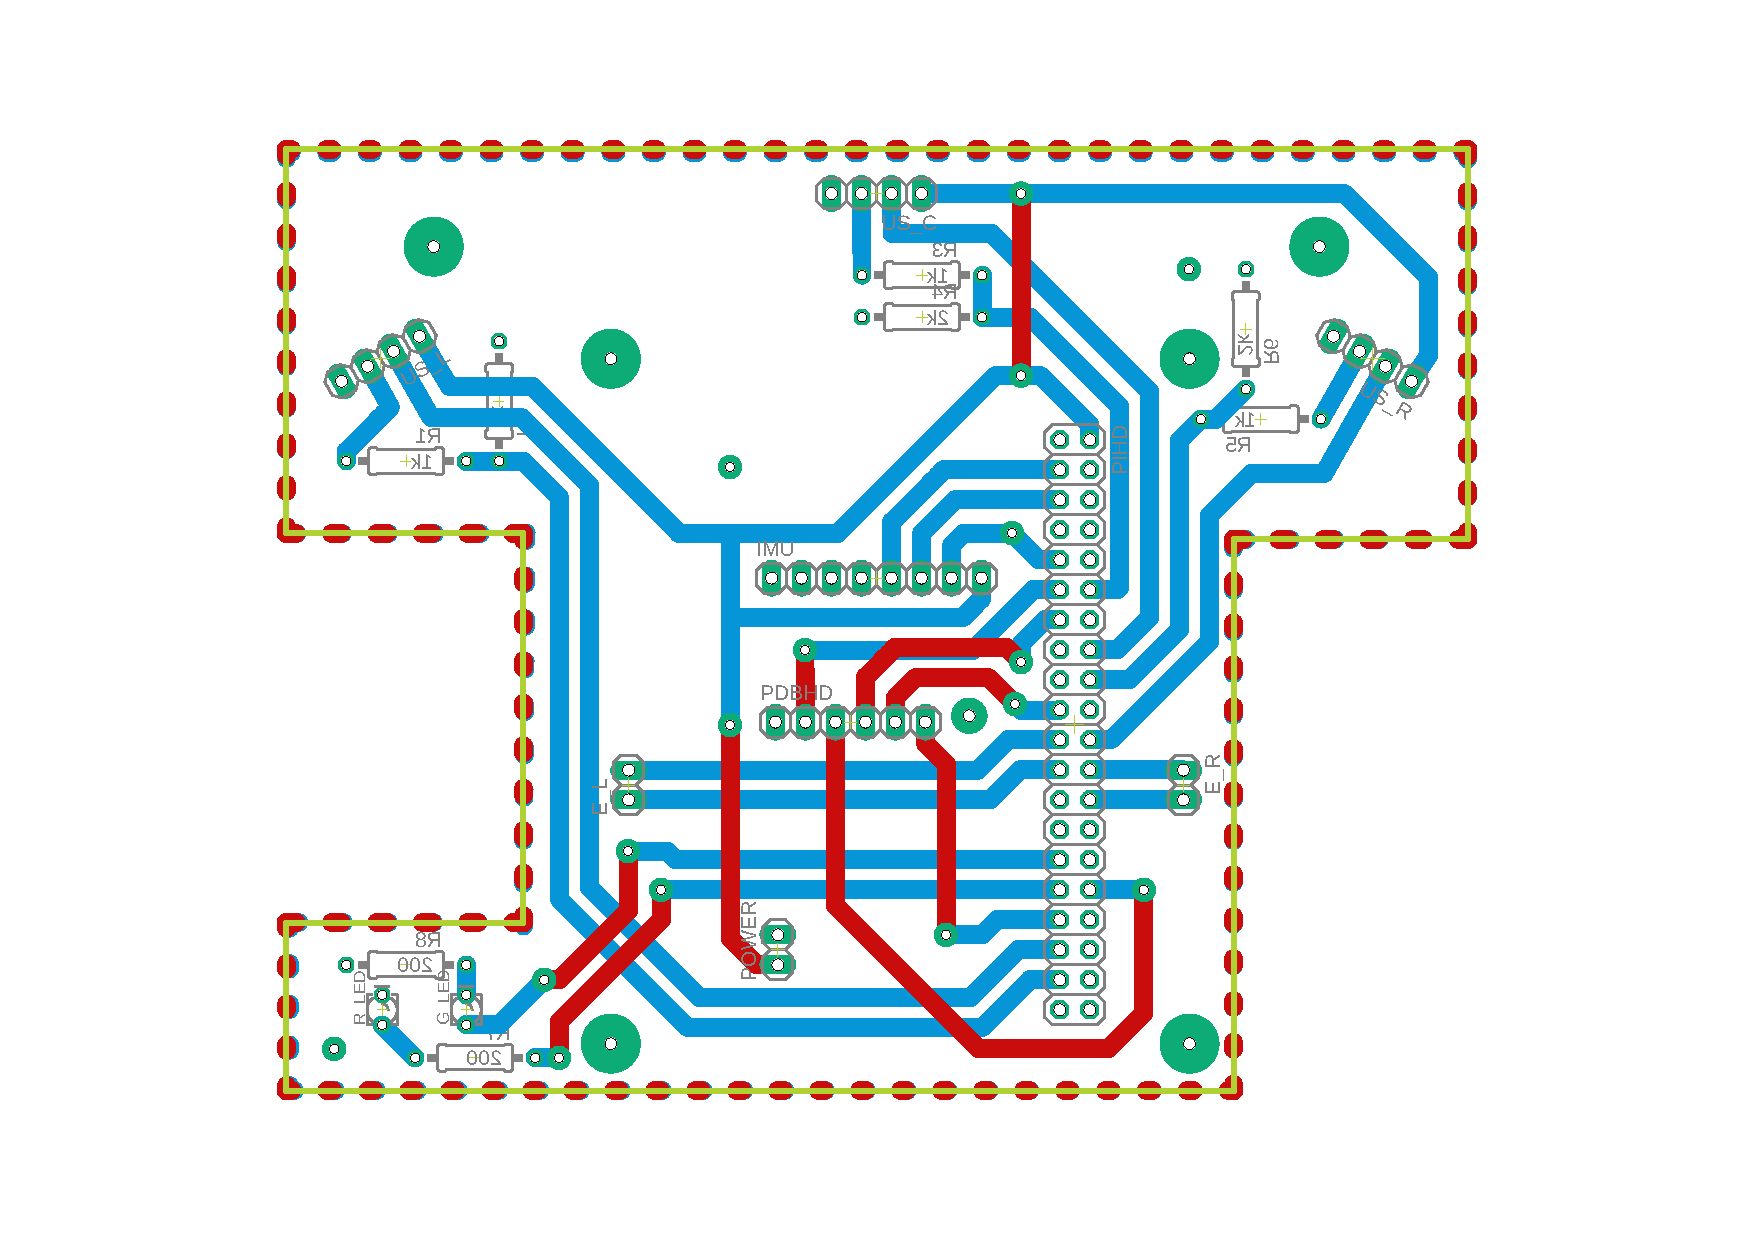
\includegraphics[width=1\textwidth]{main_pcb.pdf}
	\caption{Final PCB Design}\label{PCB_Design}

\end{figure}
Note that the peculiar shape is to allow room for the motors and encoders.

\subsection{Testing}\label{elec/pcb/test}
After the components were soldered into place on the PCB, manual
continuity tests were performed with a multimeter to ensure that adjacent
pins had not been connected in the soldering process.

The PCB was then mounted and each module test was rerun to ensure that the
connections were all correct. This process exposed a flaw as one of the
ultrasonic sensors seemed to no longer work. After some investigation it
was noticed that the screws being used had slightly larger heads than the
screws used for mounting the test strip board and was connecting two
tracks. A rubber washer was used as temporary fix and then this was
corrected in the final PCB design.
